\scanpage{96}
les ss-groupes \deleted{$\unsure{G_3,\ Z_6,\ A_4}$}, $Z_3=A_3$, $Z_6$, ${\unsure{G|\mathfrak S|\mathcal S}}_2$, $G_3$, $D_3$, $\deleted{\unsure{G}}D_6$, correspondent $1$-$1$ aux triangles de $T$, $\boxed{\mathrm{Tr}(T)}$

les ss-groupes $Z_2$, $Z_4$, \deleted{$\unsure{D_2}$}, $\deleted{\unsure{D_4}}G_{22}$, $D_4$ \unsure{corresp|correspondent} $1$-$1$ aux carrés de $T$, $\boxed{\mathrm{Car}T}$

\noindent\rule{3.6em}{.4pt}\quad $D_2,A_4,G_4$\qquad\rule{5em}{.4pt}\quad pts de $T$\quad$\boxed{T}$

\noindent\rule{3.6em}{.4pt}\quad $Z_5,D_5$\qquad\rule{5em}{.4pt}\quad pent. de $T$\quad$\boxed{\mathrm{pent}(T)}$

\noindent\rule{3.6em}{.4pt}\quad $1,A_5,G_5$\quad sont invariants

\diagram{\begin{tikzcd}[ampersand replacement=\&,column sep=0pt,row sep=0pt]
{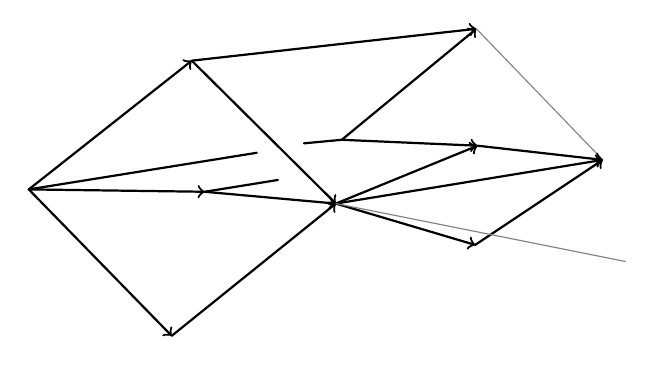
\begin{tikzpicture}[x=.015cm,y=-.015cm,line cap=round,line join=round,baseline=(current bounding box.center)]
\coordinate (l) at (17,109);
\coordinate (u) at (155,0);
\coordinate (b) at (138,233);
\coordinate (m) at (166,111);
\coordinate (r) at (277,121);
\coordinate (v) at (396,-27);
\coordinate (w) at (282,67);
\coordinate (c) at (397,72);
\coordinate (s) at (395,156);
\coordinate (z) at (503,84);
\draw[->,thick] (l)--(u);
\draw[->,thick] (u)--(r);
\draw[->,thick] (l)--(b);
\draw[->,thick] (b)--(r);
\draw[->,thick] (l)--(m);
\draw[->,thick] (m)--(r);
\draw[->,thick] (u)--(v);
\draw[->,thick] (w)--(v);
\draw[-,gray] (v)--(z);
\draw[->,thick] (w)--(c);
\draw[->,thick] (c)--(z);
\draw[->,thick] (r)--(c);
\draw[->,thick] (r)--(z);
\draw[->,thick] (r)--(s);
\draw[->,thick] (s)--(z);
\draw[thick] (l)--(210,78) (m)--(228,101) (w)--(250,70);
\draw[thin,gray] (r)--(522,170);
\end{tikzpicture}}
\end{tikzcd}}
Il y a $160$ ss-gpes $\ne 1,G_5$
\[
\begin{aligned}
\text{Nb de ss-gpes}\qquad &6\times10=60\\
+{}&4\times15=60\\
+{}&3\times5=15\\
+{}&2\times\deleted{\unsure{G_4}}12=24\\
+{}&\underline{3\times1=\phantom{2}3}\\
&\hphantom{3\times 1={}}162
\end{aligned}
\]
% crop-candidate: scan 96
\figure{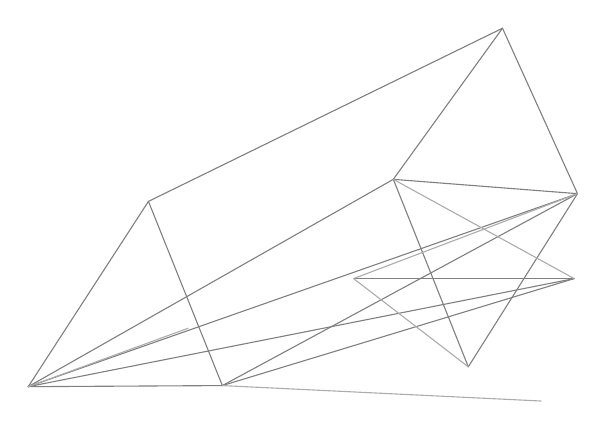
\begin{tikzpicture}[x=.014cm,y=-.014cm,line cap=round,line join=round,baseline=(current bounding box.center)]
\coordinate (l) at (0,325);
\coordinate (u) at (109,157);
\coordinate (r) at (176,324);
\coordinate (a) at (430,0);
\coordinate (b) at (331,137);
\coordinate (c) at (498,150);
\coordinate (d) at (399,307);
\coordinate (e) at (495,227);
\coordinate (f) at (295,227);
\draw[-,gray] (l)--(u);
\draw[-,gray] (u)--(r);
\draw[-,gray] (r)--(l);
\draw[-,gray] (u)--(a);
\draw[-,gray] (a)--(c);
\draw[-,gray] (c)--(b);
\draw[-,gray] (b)--(a);
\draw[-,gray] (b)--(d);
\draw[-,gray] (d)--(c);
\draw[-,gray] (l)--(b);
\draw[-,gray] (l)--(c);
\draw[-,gray] (r)--(c);
\draw[-,gray] (r)--(e);
\draw[-,gray] (e)--(f);
\draw[-,gray] (f)--(e);
\draw[-,gray] (l)--(e);
\draw[gray!65] (r)--(465,338) (f)--(d) (f)--(c) (b)--(e) (l)--(145,272);
\end{tikzpicture}}
\margin{\tikz[baseline=(n.base)]{\node[align=center] (n) {déterminer les\\ centralisateurs\\ d'éléments du\\ groupe $G_5$};\draw (n.north east) .. controls +(35:.3) and +(40:.5) .. (n.south east) .. controls +(-130:.6) and +(-70:.4) .. (n.south) .. controls +(145:.6) and +(-70:.6) .. (n.west) .. controls +(95:.5) and +(90:.3) .. (n.north east);}}
\diagram{\begin{tikzcd}[ampersand replacement=\&,column sep=0pt,row sep=0pt]
{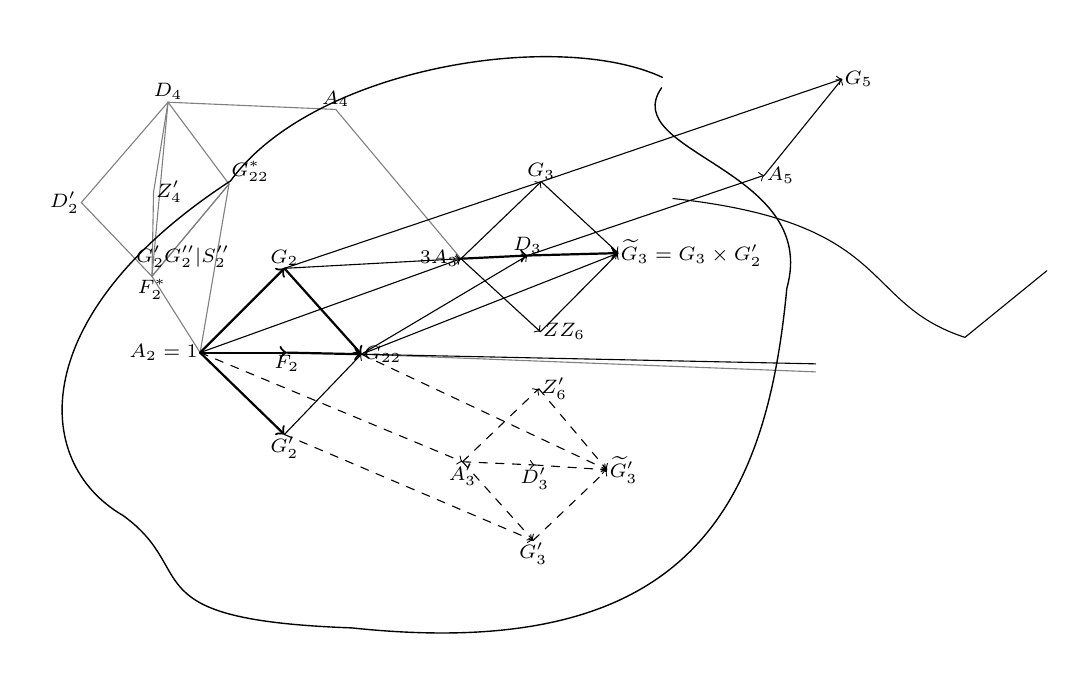
\begin{tikzpicture}[x=.0102cm,y=-.0102cm,line cap=round,line join=round,baseline=(current bounding box.center)]
\coordinate (D) at (165,788);
\coordinate (p) at (57,913);
\coordinate (z) at (147,900);
\coordinate (kk) at (145,1005);
\coordinate (sstar) at (241,890);
\coordinate (Al) at (374,797);
\coordinate (one) at (205,1100);
\coordinate (g) at (310,995);
\coordinate (f) at (313,1100);
\coordinate (gp) at (310,1202);
\coordinate (v) at (406,1102);
\coordinate (a) at (530,983);
\coordinate (h) at (630,887);
\coordinate (d) at (613,979);
\coordinate (zz) at (629,1074);
\coordinate (k) at (726,976);
\coordinate (ap) at (532,1236);
\coordinate (dp) at (622,1240);
\coordinate (zp) at (627,1145);
\coordinate (hp) at (620,1334);
\coordinate (kp) at (712,1246);
\coordinate (A) at (908,879);
\coordinate (G) at (1005,759);
\draw[-,gray] (D)--(p);
\draw[-,gray] (p)--(kk);
\draw[-,gray] (kk)--(D);
\draw[-,gray] (D)--(z);
\draw[-,gray] (z)--(kk);
\draw[-,gray] (D)--(sstar);
\draw[-,gray] (sstar)--(kk);
\draw[-,gray] (kk)--(one);
\draw[-,gray] (sstar)--(one);
\draw[-,gray] (D)--(Al);
\draw[-,gray] (kk)--(sstar);
\draw[-,gray] (Al)--(a);
\draw[->,thick] (one)--(g);
\draw[->,thick] (g)--(v);
\draw[->,thick] (one)--(f);
\draw[->,thick] (f)--(v);
\draw[->,thick] (one)--(gp);
\draw[->] (gp)--(v);
\draw[thin] (g)--(h);
\draw[->] (v)--(k);
\draw[->] (a)--(h);
\draw[->] (h)--(k);
\draw[->,thick] (a)--(d);
\draw[->,thick] (d)--(k);
\draw[->] (a)--(zz);
\draw[->] (zz)--(k);
\draw[->] (one)--(a);
\draw[->] (g)--(a);
\draw[->] (v)--(d);
\draw[->] (d)--(A);
\draw[->] (h)--(G);
\draw[->] (A)--(G);
\draw[dashed,->] (one)--(ap);
\draw[dashed,->] (gp)--(hp);
\draw[dashed,->] (v)--(kp);
\draw[dashed,->] (ap)--(hp);
\draw[dashed,->] (hp)--(kp);
\draw[dashed,->] (ap)--(dp);
\draw[dashed,->] (dp)--(kp);
\draw[dashed,->] (ap)--(zp);
\draw[dashed,->] (zp)--(kp);
\draw[gray] (v)--(972,1124);
\draw[thin] (v)--(972,1114);
\draw[line width=.5pt] (781,757) .. controls (650,696) and (345,745) .. (243,886) .. controls (-9,1050) and (-8,1235) .. (109,1303) .. controls (206,1373) and (115,1433) .. (394,1443) .. controls (810,1487) and (910,1297) .. (936,1020) .. controls (978,871) and (724,851) .. (780,770);
\draw[thin] (1158,1081) .. controls (1026,1038) and (1072,938) .. (794,908) (1158,1081)--(1260,998);
\node[anchor=south,inner sep=.7pt,font=\scriptsize] at (D) {$D_4$};
\node[anchor=east,inner sep=.7pt,font=\scriptsize] at (p) {$D'_2$};
\node[anchor=west,inner sep=.7pt,font=\scriptsize] at (z) {$Z'_4$};
\node[anchor=north,inner sep=.7pt,font=\scriptsize] at (kk) {$\mathbb F_2^*$};
\node[anchor=south west,inner sep=.7pt,font=\scriptsize] at (sstar) {$G_{22}^*$};
\node[anchor=south,inner sep=.7pt,font=\scriptsize] at (Al) {$A_4$};
\node[anchor=east,inner sep=.7pt,font=\scriptsize] at (one) {$A_2=1$};
\node[anchor=south,inner sep=.7pt,font=\scriptsize] at (g) {$G_2$};
\node[anchor=east,inner sep=.7pt,font=\scriptsize] at (245,981) {$\unsure{G'_2G''_2|\mathfrak S''_2}$};
\node[anchor=north,inner sep=.7pt,font=\scriptsize] at (f) {$F_2$};
\node[anchor=north,inner sep=.7pt,font=\scriptsize] at (gp) {$G'_2$};
\node[anchor=west,inner sep=.7pt,font=\scriptsize] at (v) {$G_{22}$};
\node[anchor=east,inner sep=.7pt,font=\scriptsize] at (a) {$\deleted{\unsure{3}}A_3$};
\node[anchor=south,inner sep=.7pt,font=\scriptsize] at (h) {$G_3$};
\node[anchor=south,inner sep=.7pt,font=\scriptsize] at (d) {$D_3$};
\node[anchor=west,inner sep=.7pt,font=\scriptsize] at (zz) {$\deleted{\unsure{Z}}Z_6$};
\node[anchor=west,inner sep=.7pt,font=\scriptsize] at (k) {$\widetilde G_3=G_3\times G'_2$};
\node[anchor=north,inner sep=.7pt,font=\scriptsize] at (ap) {$A'_3$};
\node[anchor=north,inner sep=.7pt,font=\scriptsize] at (dp) {$D'_3$};
\node[anchor=west,inner sep=.7pt,font=\scriptsize] at (zp) {$Z'_6$};
\node[anchor=north,inner sep=.7pt,font=\scriptsize] at (hp) {$G'_3$};
\node[anchor=west,inner sep=.7pt,font=\scriptsize] at (kp) {$\widetilde G'_3$};
\node[anchor=west,inner sep=.7pt,font=\scriptsize] at (A) {$A_5$};
\node[anchor=west,inner sep=.7pt,font=\scriptsize] at (G) {$G_5$};
\end{tikzpicture}}
\end{tikzcd}}
\[
\boxed{\begin{aligned} Z_2&\simeq G_2\\ D_2&\simeq G_{2,2}\\ D_3&\simeq G_3\end{aligned}}
\]
\figure{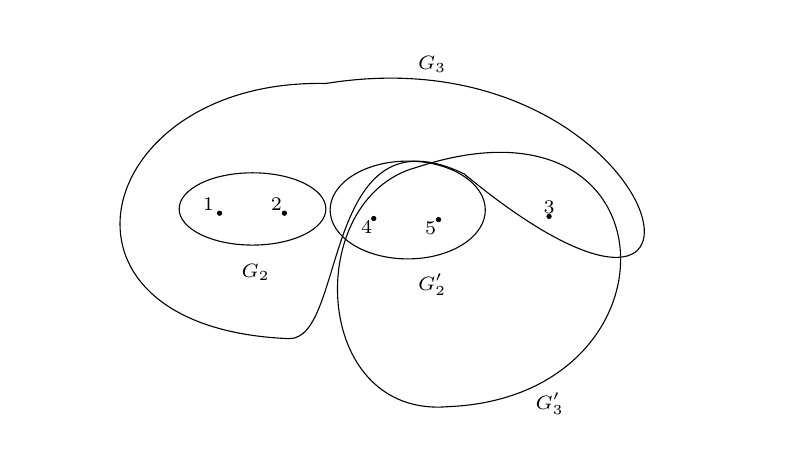
\begin{tikzpicture}[x=1.35cm,y=-1.35cm,line cap=round,line join=round,baseline=(current bounding box.center)]
\draw (1.5,1.1) .. controls (-.7,1.05) and (-1.3,3.4) .. (1.15,3.5) .. controls (1.7,3.52) and (1.45,1.3) .. (2.8,1.95) .. controls (5.65,4.3) and (4.7,.58) .. (1.5,1.1);
\draw (2.35,1.89) .. controls (1.28,2.18) and (1.36,4.25) .. (2.65,4.14) .. controls (4.9,4.05) and (4.82,1.07) .. (2.35,1.89);
\draw (.81,2.28) ellipse (.69 and .34) (2.27,2.29) ellipse (.73 and .46);
\foreach \x/\y in {.5/2.32,1.11/2.32,1.95/2.37,2.56/2.38,3.6/2.35}{\fill (\x,\y) circle (.025);}
\node[anchor=south east,inner sep=.7pt,font=\scriptsize] at (.47,2.32) {$1$};
\node[anchor=south east,inner sep=.7pt,font=\scriptsize] at (1.11,2.32) {$2$};
\node[anchor=north east,inner sep=.7pt,font=\scriptsize] at (1.96,2.37) {$4$};
\node[anchor=north east,inner sep=.7pt,font=\scriptsize] at (2.56,2.38) {$5$};
\node[anchor=south,inner sep=.7pt,font=\scriptsize] at (3.6,2.35) {$3$};
\node[anchor=south,inner sep=.7pt,font=\scriptsize] at (2.5,1.02) {$G_3$};
\node[anchor=north,inner sep=.7pt,font=\scriptsize] at (.84,2.78) {$G_2$};
\node[anchor=north,inner sep=.7pt,font=\scriptsize] at (2.5,2.87) {$G'_2$};
\node[anchor=north west,inner sep=.7pt,font=\scriptsize] at (3.45,3.99) {$G'_3$};
\end{tikzpicture}}
\[
\begin{aligned}
&\underline{1}\\
&\deleted{\unsure{G_2}}\quad\unsure{\rotatebox{90}{$=$}}\\
&Z_2\quad Z_3\quad Z_4\quad Z_5\quad Z_6\\
&D_2\quad D_3\quad D_4\quad D_5\\
&\underset{G_{2,2}}{\rotatebox{90}{$\simeq$}}\quad
 \underset{\deleted{\unsure{G_3}}}{\rotatebox{90}{$\simeq$}}\quad
 \deleted{\unsure{G_4,\ G_5}}\\
&\deleted{A_4,\ G_4,\ A_5,\ G_5}\\
&\deleted{\widetilde G_3=G_3\times}\quad A_4\quad A_5
\end{aligned}
\]
\diagram{\begin{tikzcd}[ampersand replacement=\&,column sep=0pt,row sep=0pt]
{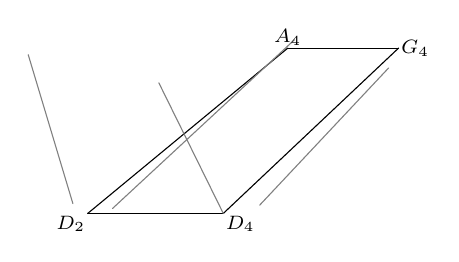
\begin{tikzpicture}[x=.021cm,y=-.021cm,line cap=round,line join=round,baseline=(current bounding box.center)]
\coordinate (D) at (0,100);
\coordinate (d) at (82,100);
\coordinate (a) at (121,0);
\coordinate (s) at (188,0);
\draw[thin] (D)--(d);
\draw[thin] (d)--(s);
\draw[thin] (s)--(a);
\draw[thin] (a)--(D);
\draw[gray] (15,97)--(125,-5) (104,95)--(182,12) (-9,94)--(-36,4) (d)--(43,21);
\node[anchor=north east,inner sep=.7pt,font=\scriptsize] at (D) {$D_2$};
\node[anchor=north west,inner sep=.7pt,font=\scriptsize] at (d) {$D_4$};
\node[anchor=south,inner sep=.7pt,font=\scriptsize] at (a) {$A_4$};
\node[anchor=west,inner sep=.7pt,font=\scriptsize] at (s) {$G_4$};
\end{tikzpicture}}
\end{tikzcd}}
\diagram{\begin{tikzcd}[ampersand replacement=\&,column sep=0pt,row sep=0pt]
{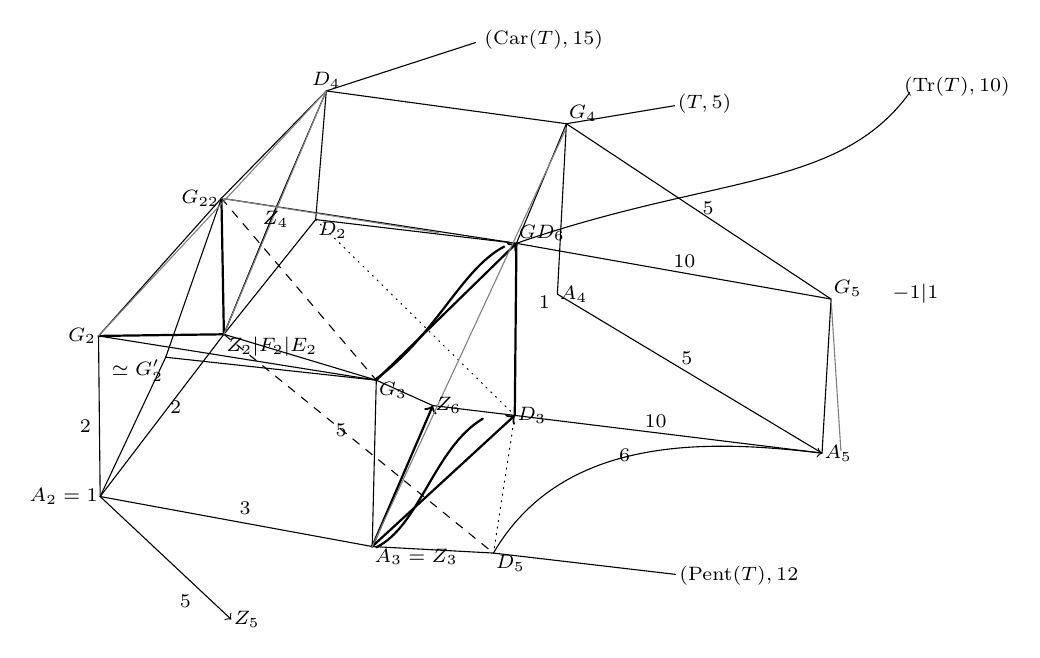
\begin{tikzpicture}[x=.0104cm,y=-.0104cm,line cap=round,line join=round,baseline=(current bounding box.center)]
\coordinate (D4) at (523,1699);
\coordinate (G4) at (816,1739);
\coordinate (V) at (395,1830);
\coordinate (Z4) at (461,1843);
\coordinate (D2) at (510,1856);
\coordinate (D6) at (755,1885);
\coordinate (G2) at (245,1998);
\coordinate (G2p) at (327,2024);
\coordinate (Z2) at (398,1996);
\coordinate (G3) at (584,2052);
\coordinate (Z6) at (653,2083);
\coordinate (D3) at (753,2095);
\coordinate (A4) at (805,1947);
\coordinate (G5) at (1139,1953);
\coordinate (A5) at (1128,2141);
\coordinate (A2) at (247,2194);
\coordinate (A3) at (579,2255);
\coordinate (D5) at (727,2263);
\coordinate (Z5) at (407,2344);
\draw[thin] (D4)--(G4);
\draw[thin] (D4)--(V);
\draw[thin] (V)--(G2);
\draw[thin] (D4)--(Z4);
\draw[thin] (Z4)--(Z2);
\draw[thin] (D4)--(D2);
\draw[thin] (D2)--(Z2);
\draw[thin] (V)--(G2p);
\draw[thin] (G2p)--(A2);
\draw[thin] (Z4)--(Z2);
\draw[-,thick] (V)--(Z2);
\draw[thin] (V)--(D6);
\draw[thin] (D2)--(D6);
\draw[dotted] (D2)--(D3);
\draw[thin] (G4)--(D6);
\draw[thin] (G4)--(A4);
\draw[thin] (G4)--(G5);
\draw[thin] (G5)--(A5);
\draw[thin] (D6)--(G5);
\draw[thin] (A4)--(A5);
\draw[thin] (D3)--(A5);
\draw[-,thick] (G2)--(Z2);
\draw[thin] (G2)--(G3);
\draw[thin] (G3)--(A3);
\draw[thin] (G2p)--(G3);
\draw[thin] (G2)--(A2);
\draw[thin] (A2)--(A3);
\draw[thin] (Z2)--(A2);
\draw[thin] (Z2)--(G3);
\draw[dashed] (Z2)--(D5);
\draw[dashed] (V)--(G3);
\draw[->,thick] (G3)--(D6);
\draw[-,thick] (D6)--(D3);
\draw[thin] (G3)--(Z6);
\draw[thin] (Z6)--(D3);
\draw[->,thick] (A3)--(Z6);
\draw[->,thick] (A3)--(D3);
\draw[thin] (A3)--(D5);
\draw[dotted] (D3)--(D5);
\draw[->] (A2)--(Z5);
\draw[->] (D5) .. controls (812,2117) and (991,2125) .. (A5);
\draw (D4)--(705,1640) (G4)--(948,1717) (D6) .. controls (997,1801) and (1149,1820) .. (1235,1701);
\draw (D5)--(949,2289);
\draw[thin,gray] (G2)--(D4) (V)--(660,1872) (A3)--(816,1744) (Z2)--(D4) (G5)--(1151,2138);
\draw[thick] (584,2256)..controls (637,2230) and (655,2134)..(714,2099) (583,2051)..controls(658,1996)and(688,1916)..(740,1889);
\node[anchor=south,inner sep=.7pt,font=\scriptsize] at (D4) {$\boxed{D_4}$};
\node[anchor=south west,inner sep=.7pt,font=\scriptsize] at (G4) {$\boxed{G_4}$};
\node[anchor=east,inner sep=.7pt,font=\scriptsize] at (V) {$G_{22}$};
\node[anchor=north,inner sep=.7pt,font=\scriptsize] at (Z4) {$Z_4$};
\node[anchor=north west,inner sep=.7pt,font=\scriptsize] at (D2) {$D_2$};
\node[anchor=south west,inner sep=.7pt,font=\scriptsize] at (D6) {$\boxed{\deleted{\unsure{G}}D_6}$};
\node[anchor=east,inner sep=.7pt,font=\scriptsize] at (G2) {$G_2$};
\node[anchor=north east,inner sep=.7pt,font=\scriptsize] at (G2p) {$\simeq G'_2$};
\node[anchor=north west,inner sep=.7pt,font=\scriptsize] at (Z2) {$\unsure{\mathbb Z_2|F_2|\mathbb E_2}$};
\node[anchor=north west,inner sep=.7pt,font=\scriptsize] at (G3) {$G_3$};
\node[anchor=west,inner sep=.7pt,font=\scriptsize] at (Z6) {$Z_6$};
\node[anchor=west,inner sep=.7pt,font=\scriptsize] at (D3) {$D_3$};
\node[anchor=west,inner sep=.7pt,font=\scriptsize] at (A4) {$A_4$};
\node[anchor=south west,inner sep=.7pt,font=\scriptsize] at (G5) {$\boxed{G_5}$};
\node[anchor=east,inner sep=.7pt,font=\scriptsize] at (1273,1947) {$\unsure{-1|1}$};
\node[anchor=west,inner sep=.7pt,font=\scriptsize] at (A5) {$A_5$};
\node[anchor=east,inner sep=.7pt,font=\scriptsize] at (A2) {$A_2=\boxed{1}$};
\node[anchor=north west,inner sep=.7pt,font=\scriptsize] at (A3) {$A_3=Z_3$};
\node[anchor=north west,inner sep=.7pt,font=\scriptsize] at (D5) {$\boxed{D_5}$};
\node[anchor=west,inner sep=.7pt,font=\scriptsize] at (Z5) {$Z_5$};
\node[anchor=west,inner sep=.7pt,font=\scriptsize] at (713,1636) {$(\mathrm{Car}(T),15)$};
\node[anchor=west,inner sep=.7pt,font=\scriptsize] at (949,1714) {$(T,5)$};
\node[anchor=west,inner sep=.7pt,font=\scriptsize] at (1225,1694) {$(\mathrm{Tr}(T),10)$};
\node[anchor=west,inner sep=.7pt,font=\scriptsize] at (951,2290) {$(\mathrm{Pent}(T),12$};
\node[anchor=center,inner sep=.7pt,font=\scriptsize] at (989,1842) {$5$};
\node[anchor=center,inner sep=.7pt,font=\scriptsize] at (960,1907) {$10$};
\node[anchor=center,inner sep=.7pt,font=\scriptsize] at (963,2025) {$5$};
\node[anchor=center,inner sep=.7pt,font=\scriptsize] at (925,2102) {$10$};
\node[anchor=north,inner sep=.7pt,font=\scriptsize] at (887,2133) {$6$};
\node[anchor=center,inner sep=.7pt,font=\scriptsize] at (789,1957) {$1$};
\node[anchor=center,inner sep=.7pt,font=\scriptsize] at (229,2108) {$2$};
\node[anchor=center,inner sep=.7pt,font=\scriptsize] at (339,2085) {$2$};
\node[anchor=center,inner sep=.7pt,font=\scriptsize] at (541,2113) {$5$};
\node[anchor=center,inner sep=.7pt,font=\scriptsize] at (424,2208) {$3$};
\node[anchor=center,inner sep=.7pt,font=\scriptsize] at (351,2322) {$5$};
\end{tikzpicture}}
\end{tikzcd}}
\[
\begin{array}{c|ccccc}
Z_1&\underline{Z_2}&\overset{A_3}{\underline{Z_3}}&\underline{Z_4}&\underline{Z_5}&\underline{Z_6}\\
\deleted{\unsure{D_1}}&\underline{D_2}&\underline{D_3}&\underline{D_4}&\underline{D_5}&\underline{D_6}\\
\deleted{\unsure{G_1}}&\underline{G_2}&\underline{G_3}&\underline{G_4}&\underline{G_5}&\\
\deleted{\unsure{A_1}}&\underline{1}=A_2&\underline{A_3}\mathrel{\rotatebox{45}{$=$}} Z_3&
 \underline{A_4},&\underline{A_5}&
\end{array}
\]
\[
\begin{aligned}
&G_{22}\\
&G''_2\times Z_2\quad \deleted{\unsure{\widetilde G_3=G_3\times|\mathfrak S_3\times}}\mathbb Z_2
\end{aligned}
\]
% archive sheet number: 95
